% Note that the a4paper option is mainly intended so that authors in
% countries using A4 can easily print to A4 and see how their papers will
% look in print - the typesetting of the document will not typically be
% affected with changes in paper size (but the bottom and side margins will).
% Use the testflow package mentioned above to verify correct handling of
% both paper sizes by the user's LaTeX system.
%
% Also note that the "draftcls" or "draftclsnofoot", not "draft", option
% should be used if it is desired that the figures are to be displayed in
% draft mode.
%
\documentclass[a4paper,12pt]{report}
\linespread{1.5} \setlength{\parskip}{0.3cm}
% Add the compsoc option for Computer Society conferences.
%
% If IEEEtran.cls has not been installed into the LaTeX system files,
% manually specify the path to it like:
% \documentclass[conference]{../sty/IEEEtran}
\usepackage{enumitem}
\usepackage{amssymb}
\usepackage{amsmath}
\usepackage{amsthm}
\usepackage{latexsym}
\usepackage{algorithm}
\usepackage{algpseudocode}
\usepackage{graphicx} 
\usepackage{tabularx,array}
\usepackage{amsfonts}
\usepackage{amsmath}
\usepackage{epsfig}
\usepackage{verbatim}
\usepackage{wallpaper}
\usepackage[skins]{tcolorbox}
\usepackage{color}
%\usepackage[export]{adjustbox}
\CenterWallPaper{.35}{figures/ccu.jpg} % Will be restored in the final thesis
\newcommand{\red}[1] {{\color{red} #1}}
%\newcommand{\blue}[1] {{\color{blue} #1}}
% Some very useful LaTeX packages include:
% (uncomment the ones you want to load)
% *** MISC UTILITY PACKAGES ***
%
%\usepackage{ifpdf}
% Heiko Oberdiek's ifpdf.sty is very useful if you need conditional
% compilation based on whether the output is pdf or dvi.
% usage:
% \ifpdf
%   % pdf code
% \else
%   % dvi code
% \fi
% The latest version of ifpdf.sty can be obtained from:
% http://www.ctan.org/tex-archive/macros/latex/contrib/oberdiek/
% Also, note that IEEEtran.cls V1.7 and later provides a builtin
% \ifCLASSINFOpdf conditional that works the same way.
% When switching from latex to pdflatex and vice-versa, the compiler may
% have to be run twice to clear warning/error messages.


% *** CITATION PACKAGES ***
%
\usepackage{cite}
\usepackage{ulem}
% cite.sty was written by Donald Arseneau
% V1.6 and later of IEEEtran pre-defines the format of the cite.sty package
% \cite{} output to follow that of IEEE. Loading the cite package will
% result in citation numbers being automatically sorted and properly
% "compressed/ranged". e.g., [1], [9], [2], [7], [5], [6] without using
% cite.sty will become [1], [2], [5]--[7], [9] using cite.sty. cite.sty's
% \cite will automatically add leading space, if needed. Use cite.sty's
% noadjust option (cite.sty V3.8 and later) if you want to turn this off.
% cite.sty is already installed on most LaTeX systems. Be sure and use
% version 4.0 (2003-05-27) and later if using hyperref.sty. cite.sty does
% not currently provide for hyperlinked citations.
% The latest version can be obtained at:
% http://www.ctan.org/tex-archive/macros/latex/contrib/cite/
% The documentation is contained in the cite.sty file itself.
\usepackage{amsmath}
\usepackage{longtable}
\newcommand{\tabincell}[2]{\begin{tabular}{@{}#1@{}}#2\end{tabular}}%放在导言区 



% *** GRAPHICS RELATED PACKAGES ***
%
%\ifCLASSINFOpdf
 %  \usepackage[pdftex]{graphicx}
  % declare the path(s) where your graphic files are
  % \graphicspath{{../pdf/}{../jpeg/}}
  % and their extensions so you won't have to specify these with
  % every instance of \includegraphics
  % \DeclareGraphicsExtensions{.pdf,.jpeg,.png}
%\else
  % or other class option (dvipsone, dvipdf, if not using dvips). graphicx
  % will default to the driver specified in the system graphics.cfg if no
  % driver is specified.
 %  \usepackage[dvips]{graphicx}
  % declare the path(s) where your graphic files are
  % \graphicspath{{../eps/}}
  % and their extensions so you won't have to specify these with
  % every instance of \includegraphics
  % \DeclareGraphicsExtensions{.eps}
%\fi
% graphicx was written by David Carlisle and Sebastian Rahtz. It is
% required if you want graphics, photos, etc. graphicx.sty is already
% installed on most LaTeX systems. The latest version and documentation can
% be obtained at:
% http://www.ctan.org/tex-archive/macros/latex/required/graphics/
% Another good source of documentation is "Using Imported Graphics in
% LaTeX2e" by Keith Reckdahl which can be found as epslatex.ps or
% epslatex.pdf at: http://www.ctan.org/tex-archive/info/
%
% latex, and pdflatex in dvi mode, support graphics in encapsulated
% postscript (.eps) format. pdflatex in pdf mode supports graphics
% in .pdf, .jpeg, .png and .mps (metapost) formats. Users should ensure
% that all non-photo figures use a vector format (.eps, .pdf, .mps) and
% not a bitmapped formats (.jpeg, .png). IEEE frowns on bitmapped formats
% which can result in "jaggedy"/blurry rendering of lines and letters as
% well as large increases in file sizes.
%
% You can find documentation about the pdfTeX application at:
% http://www.tug.org/applications/pdftex



\usepackage{float}

% *** MATH PACKAGES ***
%
%\usepackage[cmex10]{amsmath}
% A popular package from the American Mathematical Society that provides
% many useful and powerful commands for dealing with mathematics. If using
% it, be sure to load this package with the cmex10 option to ensure that
% only type 1 fonts will utilized at all point sizes. Without this option,
% it is possible that some math symbols, particularly those within
% footnotes, will be rendered in bitmap form which will result in a
% document that can not be IEEE Xplore compliant!
%
% Also, note that the amsmath package sets \interdisplaylinepenalty to 10000
% thus preventing page breaks from occurring within multiline equations. Use:
%\interdisplaylinepenalty=2500
% after loading amsmath to restore such page breaks as IEEEtran.cls normally
% does. amsmath.sty is already installed on most LaTeX systems. The latest
% version and documentation can be obtained at:
% http://www.ctan.org/tex-archive/macros/latex/required/amslatex/math/


% *** SPECIALIZED LIST PACKAGES ***
%
%\usepackage{algorithmic}
% algorithmic.sty was written by Peter Williams and Rogerio Brito.
% This package provides an algorithmic environment fo describing algorithms.
% You can use the algorithmic environment in-text or within a figure
% environment to provide for a floating algorithm. Do NOT use the algorithm
% floating environment provided by algorithm.sty (by the same authors) or
% algorithm2e.sty (by Christophe Fiorio) as IEEE does not use dedicated
% algorithm float types and packages that provide these will not provide
% correct IEEE style captions. The latest version and documentation of
% algorithmic.sty can be obtained at:
% http://www.ctan.org/tex-archive/macros/latex/contrib/algorithms/
% There is also a support site at:
% http://algorithms.berlios.de/index.html
% Also of interest may be the (relatively newer and more customizable)
% algorithmicx.sty package by Szasz Janos:
% http://www.ctan.org/tex-archive/macros/latex/contrib/algorithmicx/




% *** ALIGNMENT PACKAGES ***
%
%\usepackage{array}
% Frank Mittelbach's and David Carlisle's array.sty patches and improves
% the standard LaTeX2e array and tabular environments to provide better
% appearance and additional user controls. As the default LaTeX2e table
% generation code is lacking to the point of almost being broken with
% respect to the quality of the end results, all users are strongly
% advised to use an enhanced (at the very least that provided by array.sty)
% set of table tools. array.sty is already installed on most systems. The
% latest version and documentation can be obtained at:
% http://www.ctan.org/tex-archive/macros/latex/required/tools/


%\usepackage{mdwmath}
%\usepackage{mdwtab}
% Also highly recommended is Mark Wooding's extremely powerful MDW tools,
% especially mdwmath.sty and mdwtab.sty which are used to format equations
% and tables, respectively. The MDWtools set is already installed on most
% LaTeX systems. The lastest version and documentation is available at:
% http://www.ctan.org/tex-archive/macros/latex/contrib/mdwtools/


% IEEEtran contains the IEEEeqnarray family of commands that can be used to
% generate multiline equations as well as matrices, tables, etc., of high
% quality.

%\usepackage{eqparbox}
% Also of notable interest is Scott Pakin's eqparbox package for creating
% (automatically sized) equal width boxes - aka "natural width parboxes".
% Available at:
% http://www.ctan.org/tex-archive/macros/latex/contrib/eqparbox/

% *** SUBFIGURE PACKAGES ***
%\usepackage[tight,footnotesize]{subfigure}
% subfigure.sty was written by Steven Douglas Cochran. This package makes it
% easy to put subfigures in your figures. e.g., "Figure 1a and 1b". For IEEE
% work, it is a good idea to load it with the tight package option to reduce
% the amount of white space around the subfigures. subfigure.sty is already
% installed on most LaTeX systems. The latest version and documentation can
% be obtained at:
% http://www.ctan.org/tex-archive/obsolete/macros/latex/contrib/subfigure/
% subfigure.sty has been superceeded by subfig.sty.

%\usepackage[caption=false]{caption}
\usepackage[font=footnotesize]{subfig}
% subfig.sty, also written by Steven Douglas Cochran, is the modern
% replacement for subfigure.sty. However, subfig.sty requires and
% automatically loads Axel Sommerfeldt's caption.sty which will override
% IEEEtran.cls handling of captions and this will result in nonIEEE style
% figure/table captions. To prevent this problem, be sure and preload
% caption.sty with its "caption=false" package option. This is will preserve
% IEEEtran.cls handing of captions. Version 1.3 (2005/06/28) and later
% (recommended due to many improvements over 1.2) of subfig.sty supports
% the caption=false option directly:
%\usepackage[caption=false,font=footnotesize]{subfig}
%
% The latest version and documentation can be obtained at:
% http://www.ctan.org/tex-archive/macros/latex/contrib/subfig/
% The latest version and documentation of caption.sty can be obtained at:
% http://www.ctan.org/tex-archive/macros/latex/contrib/caption/

% *** FLOAT PACKAGES ***
%
%\usepackage{fixltx2e}
% fixltx2e, the successor to the earlier fix2col.sty, was written by
% Frank Mittelbach and David Carlisle. This package corrects a few problems
% in the LaTeX2e kernel, the most notable of which is that in current
% LaTeX2e releases, the ordering of single and double column floats is not
% guaranteed to be preserved. Thus, an unpatched LaTeX2e can allow a
% single column figure to be placed prior to an earlier double column
% figure. The latest version and documentation can be found at:
% http://www.ctan.org/tex-archive/macros/latex/base/



%\usepackage{stfloats}
% stfloats.sty was written by Sigitas Tolusis. This package gives LaTeX2e
% the ability to do double column floats at the bottom of the page as well
% as the top. (e.g., "\begin{figure*}[!b]" is not normally possible in
% LaTeX2e). It also provides a command:
%\fnbelowfloat
% to enable the placement of footnotes below bottom floats (the standard
% LaTeX2e kernel puts them above bottom floats). This is an invasive package
% which rewrites many portions of the LaTeX2e float routines. It may not work
% with other packages that modify the LaTeX2e float routines. The latest
% version and documentation can be obtained at:
% http://www.ctan.org/tex-archive/macros/latex/contrib/sttools/
% Documentation is contained in the stfloats.sty comments as well as in the
% presfull.pdf file. Do not use the stfloats baselinefloat ability as IEEE
% does not allow \baselineskip to stretch. Authors submitting work to the
% IEEE should note that IEEE rarely uses double column equations and
% that authors should try to avoid such use. Do not be tempted to use the
% cuted.sty or midfloat.sty packages (also by Sigitas Tolusis) as IEEE does
% not format its papers in such ways.

% *** PDF, URL AND HYPERLINK PACKAGES ***
%
\usepackage{url}
% url.sty was written by Donald Arseneau. It provides better support for
% handling and breaking URLs. url.sty is already installed on most LaTeX
% systems. The latest version can be obtained at:
% http://www.ctan.org/tex-archive/macros/latex/contrib/misc/
% Read the url.sty source comments for usage information. Basically,
% \url{my_url_here}.
%\usepackage{amssymb}
%\usepackage{amsmath}
%\usepackage{amsthm}
\usepackage{latexsym}
\usepackage{graphicx}
\usepackage{array,booktabs}
\usepackage{multicol}
\usepackage{multirow}
\usepackage{tabularx}
\usepackage{textcomp}


\makeatletter
\def\@normalsize{\@setsize\normalsize{12pt}\xpt\@xpt
\abovedisplayskip 10pt plus2pt minus5pt\belowdisplayskip
\abovedisplayskip \abovedisplayshortskip \z@
plus3pt\belowdisplayshortskip 6pt plus3pt
minus3pt\let\@listi\@listI}


\def\subsize{\@setsize\subsize{12pt}\xipt\@xipt}
\def\section{\@startsection {section}{1}{\z@}{24pt plus 2pt minus 2pt}
{12pt plus 2pt minus 2pt}{\large\bf}}
\def\subsection{\@startsection {subsection}{2}{\z@}{12pt plus 2pt minus 2pt}
{12pt plus 2pt minus 2pt}{\subsize\bf}} \makeatother


% *** Do not adjust lengths that control margins, column widths, etc. ***
% *** Do not use packages that alter fonts (such as pslatex).         ***
% There should be no need to do such things with IEEEtran.cls V1.6 and later.
% (Unless specifically asked to do so by the journal or conference you plan
% to submit to, of course. )


% correct bad hyphenation here
\hyphenation{op-tical net-works semi-conduc-tor}

%\usepackage{fontspec}   				%加這個就可以設定字體
%\usepackage{xeCJK}       				%讓中英文字體分開設置
%\setCJKmainfont{標楷體} 					%設定中文為系統上的字型,而英文不去更動,使用原TeX字型
%\XeTeXlinebreaklocale "zh"             	%這兩行一定要加,中文才能自動換行
%\XeTeXlinebreakskip = 0pt plus 1pt     	%這兩行一定要加,中文才能自動換行

\begin{document}
\bibliographystyle{plain}
%
% paper title
% can use linebreaks \\ within to get better formatting as desired


% author names and affiliations
% use a multiple column layout for up to three different
% affiliations
\title{\bf Rapid Detection of Disobedient Forwarding on a Compromised OpenFlow Switch}
\author{{\bf Student: Chiu, Yen-Chun}
\\ {\bf Advisor: Prof. Lin, Po-Ching}
\\ National Chung Cheng University
\\ Ming-Hsiung, Chiayi 621, Taiwan
\\ shuaichiou@gmail.com}
\date{July, 19, 2016}

% conference papers do not typically use \thanks and this command
% is locked out in conference mode. If really needed, such as for
% the acknowledgment of grants, issue a \IEEEoverridecommandlockouts
% after \documentclass

% for over three affiliations, or if they all won't fit within the width
% of the page, use this alternative format:
%
%\author{\IEEEauthorblockN{Michael Shell\IEEEauthorrefmark{1},
%Homer Simpson\IEEEauthorrefmark{2},
%James Kirk\IEEEauthorrefmark{3},
%Montgomery Scott\IEEEauthorrefmark{3} and
%Eldon Tyrell\IEEEauthorrefmark{4}}
%\IEEEauthorblockA{\IEEEauthorrefmark{1}School of Electrical and Computer Engineering\\
%Georgia Institute of Technology,
%Atlanta, Georgia 30332--0250\\ Email: see http://www.michaelshell.org/contact.html}
%\IEEEauthorblockA{\IEEEauthorrefmark{2}Twentieth Century Fox, Springfield, USA\\
%Email: homer@thesimpsons.com}
%\IEEEauthorblockA{\IEEEauthorrefmark{3}Starfleet Academy, San Francisco, California 96678-2391\\
%Telephone: (800) 555--1212, Fax: (888) 555--1212}
%\IEEEauthorblockA{\IEEEauthorrefmark{4}Tyrell Inc., 123 Replicant Street, Los Angeles, California 90210--4321}


% use for special paper notices
%\IEEEspecialpapernotice{(Invited Paper)}




% make the title area
\maketitle

\setcounter{page}{1}
\pagenumbering{roman}
\begin{abstract}
\label{sec:abstract}
Software defined network (SDN) is a next-generation concept that allows network administrators to manage network flows a lot easier. It is programmable, centrally managed, and flexible with topology alteration. However, these new features also lead to new security problems. Applications, controllers, Openflow switches, topology managing mechanism, there are a lot of newly-introduced vectors for us to concern about. Although protection mechanisms such as TopoGuard and FortNox have been proposed, there are still more possibilities of attacks and countermeasures in different scenarios left to be discovered. Furthermore, as SDN evolves, it will definitely bring more new security issues. In this paper, we analysis possibilities of attacks when a switch is compromised and create a disobedient forwarding detection method. To enhance the detection efficiency and minimize the additional network traffic, we try to reduce the number of detection packets by aggregating the flow entries in a reasonable amount of computation time. The result of the experiment shows that XXXXXXXXXXXXXXXXXXXXXXXX
\end{abstract}
%backup=====================
%According to the profiling, we find pattern matching can dominate the execution time if the NIDS is configured to scan every packet payload in the packet traces.
%Moreover, the preprocessing stage can be heavy when the NIDS handles packet reassembly for IP segments in malicious traffic.
%Adjusting the depth of payload to be scanned in the system configuration will be effective for performance adaptation under heavy load.
%============================
% IEEEtran.cls defaults to using nonbold math in the Abstract.
% This preserves the distinction between vectors and scalars. However,
% if the conference you are submitting to favors bold math in the abstract,
% then you can use LaTeX's standard command \boldmath at the very start
% of the abstract to achieve this. Many IEEE journals/conferences frown on
% math in the abstract anyway.

%\begin{keywords}
%NIDS, adversarial network traffic, system performance, pattern matching.
%\end{keywords}

% For peer review papers, you can put extra information on the cover
% page as needed:
% \ifCLASSOPTIONpeerreview
% \begin{center} \bfseries EDICS Category: 3-BBND \end{center}
% \fi
%
% For peerreview papers, this IEEEtran command inserts a page break and
% creates the second title. It will be ignored for other modes.
%\IEEEpeerreviewmaketitle

\tableofcontents\listoffigures\listoftables
\chapter{Introduction}
\label{chap:intro}
\setcounter{page}{1}
\pagenumbering{arabic}

Nowadays, as the popularity of public clouds like Google cloud, Microsoft Azure, Amazon EC2 increase, we can see how cloud computing offers a new way of deploying applications and services. While users tend to move everything onto the clouds, handling the growth of volume and complexity of data center network (DCN) is getting challenging. Consequently, networking organizations are under increasing pressure of being more efficient, agile and maintainable. In traditional networks, implementing a network-wide policy requires configuring at the device level. The process is time-consuming, error-prone and manpower-heavy, and it is a formidable job for network administrators to manage a large network.

Software defined network (SDN) is a dynamic, programmable, cost-effective network structure that gains great popularity in the industry and academia in recent years {\color{red} Refer to some popular SDN tutorial papers here}. In SDN, a controller centrally manage a number of switches in a consistent manner, and network applications can be developed on the controller for flexible management. The controller is able to control all network flow by configuring flow rules inside the switches. Also, components of legacy network such as a regular switch is totally compatible within a SDN network structure {\color{red} Add a reference to justify this sentence}.

Nevertheless, SDN often comes with new security problems {\color{red} Refer to some popular SDN security survey papers here}. There are also some new mechanisms such as topology discovery, host management, protocols and APIs for the communication between entities. With so many new elements introduced, there will be more potential security issues that need to be taken care of in various ways. {\color{red} Briefly summarize the categories of security issues in SDN here.}

In this work, we present a method to address xxx {\color{red} The issues to be addressed in this work}. For example, in \cite{HXWG15}, Hong et al. propose attacks that poison network visibility and its countermeasure, but they did not consider the situation that switches are compromised. to the best of our knowledge, although some protection method are proposed, there has not been an effective way to detect if there is any switch being compromised in the network. With the program-configurable trait of SDN, we believe it is possible to implement defensive solution with the aids of SDN properties. We hope we are able to set an example to inspire others and draw more attention from the community to concern more about the security issues in SDN, and ultimately resulting in a more mature SDN environment.

During the research, we study the specification of components as well as the potential threats in SDN. After discussing about those attacks, we try to cover the situations that were left by others. In this work, there are \emph{two main goals}: the first one is to improve an existing switch detection method. The detection method is able to detect whether a flow entry works as expected. However, it can only detect one flow entry at a time, which does not seem to be efficient enough. To solve this problem, we try to aggregate the match fields to reduce the number of detection packets. The second goal is to propose a new detection method that is able to detect a fabricated link caused by LLDP packets manipulation. The main idea behind it is to measure the round trip time of LLDP packets. If an intermediate switch is compromised and manipulates the LLDP packet, it is very likely to increase the round trip time. Nevertheless, time measuring will be significantly influenced by traffic jam. Therefore, we implement \textit{packet pair} to deal with this problem. With two packets sent at the same time, we are able to estimate the delay of traffic crowdedness by using the arrival time of two packets.

In the experiments, we found that our method XXXXXXXXXXXXXXXXXXXXXXXXXXXXXXXXXXXXXXXXX. Finally, we will discuss about the future expectation of this work.

The \emph{main contributions of this paper} are as follow:

\begin{enumerate}
\item
Analysis several types of attacks that influence the visibility of network.
\item
Discuss about counter measurements in previous works.
\item
Improve an existing switch entry validation method.
\item
Create an innovative fake link detection method.
\item
Evaluate and discuss about our methods.
\end{enumerate}

The following chapters in this thesis will be: Chapter 2 gives detail background knowledge of the used technology, discuss about possible threats and countermeasure. Chapter 3 is about our threat model and the theory of our own detection method. XXXXXXXXXXXXXXXXXXXXXXXXXXXXXXXXXXXXXXXXX.
-----------------------------------------------
Chapter 4 contains the experimental details including setup, considerations, simulations of attacks and evaluation methods. In Chapter 5, the proposed method will be evaluated under different conditions. Finally, the conclusion and future expectation of this work will be in Chapter 6.
\chapter{Background and related work}
\section{SDN and OpenFlow}
OpenFlow is the most popular southbound interface in SDN. A switch that supports OpenFlow is called an OpenFlow switch. Aside from physical switches, there are also software implementations of virtual switches, such as \textit{Open vSwtich} (\url{openvswitch.org}). OpenFlow switches typically separate OpenFlow and non-OpenFlow traffic, which do not interfere with each other \cite{HP_SPEC}.

A controller is able to determine the forwarding path of packets by adding, updating and deleting flow entries in the flow tables of OpenFlow switches in both reactive and proactive ways \cite{OF_SPEC}. It also maintains the abstract view of the network, including network topology, host positions and the states of network resources. An incoming packet from the \textit{ingress port} will go through one or more flow tables, optionally through the group table, and be processed according to the actions defined by the matched flow entry. Each OpenFlow table typically contains thousands of flow entries. Figure~\ref{FE_Col} presents the columns of a flow entry. Packets will be matched with the \textit{match fields} of a flow entry. When a packet matches a flow entry, the action set to that packet will be modified according to the instructions in the entry. There is an entry with the lowest priority that matches all fields. It is for packets that cannot match any other flow entries. Normally, such a packet will be encapsulated and sent to the controller, which will decide how to process it and add a new flow entry according to the network policy. After the end of processing pipeline, the actions in the action set will be executed.% When ports are added or removed, the content of flow tables remain unchanged, so the controller should clean up the reference of a port if a port is deleted \cite{OF_SPEC}.

\begin{figure}[H]
\begin{center} 
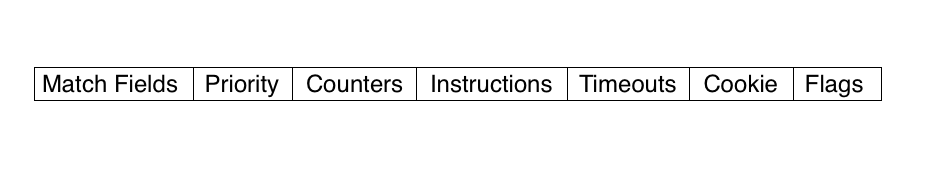
\includegraphics[width=1\textwidth]{figures/columns_of_flow_entry.png}
\end{center}
\caption{Columns of a flow entry.}
\label{FE_Col}
\end{figure}

\section{Topology discovery services}
\label{Topology discovery services}
The controller needs to maintain the visibility of the whole network to realize centralized control and high programmability. Therefore, topology discovery services play an important role in SDN. The services help to reduce manual efforts significantly when the topology is altered. The topology services include three parts: switch discovery, host tracking and internal link.

\subsection{Switch discovery service and Host tracking service}
Switch discovery is rather simple. When a switch initiates a connection with a controller, the OpenFlow channel will be established, and the switch information will be sent to the controller. A controller maintains the host profiles to keep track of the locations of hosts. When a packet-miss happens in the flow table, a \texttt{Packet\_In} message will be sent to the controller along with the packet's information and the controller will look up the host profiles it maintains. If the host profile of the host cannot be found, the controller will assume a new host joining the network and add the information of the host. If there is a conflict between the host profile and the \texttt{Packet\_In} message, the controller treats this as a host migration and updates the location in the host profile.

\subsection{Link discovery service}
\label{Link discovery service}
Link discovery refers to the procedure of discovering the links between switches. Since there has not been a standard for the link discovery in the OpenFlow controller, we will use the term \textit{OpenFlow Discovery Protocol} (OFDP) when mentioning it. Currently, all mainstream controllers support OFDP despite some minor differences in detail.

OFDP leverages the Link Layer Discovery Protocol (LLDP) with subtle modification to perform topology discovery in an OpenFlow network. LLDP is originally implemented for an Ethernet switch to exchange its identity and capabilities with adjacent layer-2 peers. In a legacy network, LLDP packets are sent regularly via each port of switches \cite{LLDP_WS}. A switch stores the information learned from LLDP packets sent by the neighbors and the packets will not be forwarded further. Figure~\ref{LLDP_frame} shows the structure of an LLDP Ethernet frame. Each LLDP data unit contains a sequence of type-length-values (TLV). 

\begin{figure}[H]
\begin{center} 
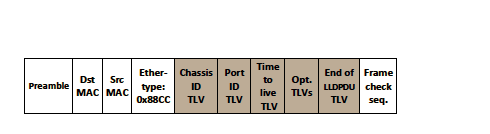
\includegraphics[width=1\textwidth]{figures/LLDP_packet_format.png}
\end{center}
\caption{LLDP packet frame structure. \cite{LLDP_WS}}
\label{LLDP_frame}
\end{figure}

However, OFDP operates quite differently. The controller keeps the topology information, and an OpenFlow switch does nothing more than forwarding the LLDP packet. The simplified process is shown in Figure~\ref{OFDP}. All switches have a pre-installed rule in their flow tables. The rule specifies to send LLDP packets received from any ports except the controller port back to controller via \texttt{Packet\_In}. Initially, the controller creates an LLDP packet for each port on every switch via the \texttt{Packet\_Out} message. After receiving the LLDP packet from controller, S1 sends it out on Port 1 and received by S2 on Port 3. With the pre-installed forwarding rule, switch S2 forwards the received LLDP packet to the controller via a \texttt{Packet\_In} message, which contains meta-data such as the identifier of the switch and the ingress port via which the packet was received. Thus, the controller can now infer that there exists a link between Port 1 of S1 and Port 3 of S2, and this information will be added to controller's topology database. After running this process through all the ports on all the switches, the controller will obtain all links between switches in the network. The entire discovery process is performed periodically with a typical default interval size of 5 seconds \cite{PPTI14}. 

\begin{figure}[H]
\begin{center} 
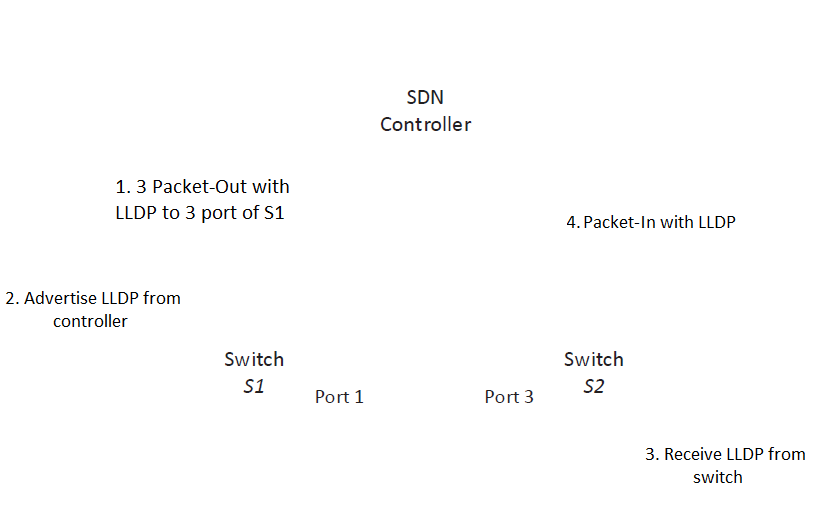
\includegraphics[width=1\textwidth]{figures/OFDP_procedure.png}
\end{center}
\caption{An illustration of OFDP procedure.}
\label{OFDP}
\end{figure}

\section{SDN security}
\label{SDN security}
As SDN brings fascinating development and introduces new factors to network technology, there are a lot more vectors for us to concern about. Figure~\ref{SND_threat_overview} is a whole picture of attacks we discuss and where they might take place inside SDN, and Table~\ref{table:sdn_threats} contains further description of these threats. In this chapter, we will talk about SDN security-related issues. We will focus on some of them and discuss about the attack scenarios, possible consequences and countermeasures. 

\begin{figure}[H]
\begin{center} 
\includegraphics[width=1\textwidth]{figures/SDN_threat_overview.png}
\end{center}
\caption{SDN threat overview.}
\label{SND_threat_overview}
\end{figure}

\begin{table}[H]
\centering
\caption{Detail of each attack.}
\begin{tabular}{|l|p{4cm}|p{3.2cm}|p{5cm}|}
\hline ID & Threat name	& Location & Consequences \\
\hline
\hline 1 & System Vulnerability & all devices & Device compromised\\
\hline 2 & Administrative Interface Compromised & all administrative interfaces & Device compromised \\
\hline 3 & Application Vulnerability & SDN application & Malicious command to controller \\
\hline 4 & Host Hijacking & host & Attacker receives target host's traffic \\
\hline 5 & Link Fabrication & link between switch & Add non-existing link to controller's view \\
\hline 6 & Flow Entry Modification & switch & Unwanted packet redirection or drop \\
\hline 7 & Malicious Packet Controller DOS  & host, switch & DOS to controller \\
\hline 8 & Control-channel Hijacking & switch & Manipulate control traffic \\
\hline 
\end{tabular}
\label{table:sdn_threats}
\end{table}

\subsection{General security}
There are quite a few devices in SDN network, such as controllers, switches and hosts. All these devices possibly contain system vulnerabilities like Heartbleeding, Poodle and Shellshock \cite{HB,POODLE,SHELLSHOCK} found in recent years. Moreover, one might be able to gain unauthorized access to the network physically or virtually, by using trivial methods like brute forcing the administrative interface or a physical break in. To deal with these kind of threats, all the best practices for hardening servers are applicable. Autonomic trust management technique should be used to harden these components in the network \cite{YZP11}. Also, Diego et al. propose replication, dynamic device association and self-healing concepts in their work to reinforce the security \cite{KDFRV13}. As to the administrative interface, organizations should implement Role-Based Access Control (RBAC) policies and event logging \cite{FFR09}. With all these methods, the damage should be reduced if controller compromise should happen.

\subsection{Topology poisoning attacks}
So far, the topology poisoning attacks have been discussed in many papers. The main idea of this type of attack is to trick controller into believing the existence of a non-existing link to host or switch by exploiting traits of topology management service. One can initiate such type of attack with either a switch or a host.

In Host Location Hijacking Attack, attacker exploits the trait of Host Tracking Service. The attacker impersonates a target host by sending spoofed packet with the host's information with PACKET\_IN, and the controller will think that the target host has moved to a new location. But the truth is, the traffic of the target host is now redirected to the attacker's host \cite{HXWG15}. Another type of host-initiated attack is called Link Fabrication Attack. The attack is caused by the fact that OpenFlow controllers accept LLDP from all switch ports, even if it is connected to a host. After an attacker receives LLDP packet with a host, he can modify specific contents like DPID or port number of LLDP packets to launch a LLDP packet injection attack. To deal with these two types of host-initiated attack, Hong et al. present TopoGuard, a new security extension to OpenFlow controller. They verify the legitimacy of Host Migration by further inspecting sign of host migration, and manage port property in order to avoid any host residing inside the LLDP propagation \cite{HXWG15}.

However, LLDP packets are passed around with the aid of switches. The Link Fabrication Attack can also initiate by compromised switches, which is not included in the scenario of TopoGuard. Bui gives three different attack scenarios of Link Fabrication Attack with compromised switches, which are two-switch tunnel attack extended two-switch tunnel attack and single-switch attack, and evaluates their consequence under different routing algorithms and network topologies \cite{TTB15}. This attack is caused by the lack of authentication of LLDP. However, simply adding authenticator inside LLDP packet will not help against LLDP relay attack \cite{HXWG15}. Alharbi et al. implement HMAC based mechanism with a little modification to static secret key, which is able to detect the injection of any fabricated LLDP packets, with only an acceptable of amount of overhead added \cite{ATPP15}.

Besides link fabrication attacks, attackers can also modify the flow entries inside the flow tables of the compromised switch to perform MITM, eavesdropping or DOS attack \cite{AAS14}. The detection method proposed in \cite{CKGL15} is able to detect whether a switch is forwarding the packets in an unexpected way. After selecting a flow entry as the detecting target, they install new entry on its neighbors. With the match field selected by their algorithm, they are able to let every packet that matches the new flow entry matches the target flow entry. A packet containing the match field of the new flow entry will be sent from Packet\_Out to a neighbor of the target switch, forwarded to the target switch, and should be sent back to the controller. Finally, they will check if the packet comes back to the controller as expected and remain unchanged. However, this method will take a longer time to run if we want to scan through lots of flow entries. Pre-detection method to narrow down the potential target is needed.

\chapter{Detection Algorithm}
This work focuses on the problem that a compromised switch will bring and presents the method to detect such a switch. Our method emphasizes on scanning through the whole network with fewer packets and high detection efficiency. In this chapter, we will define the threat models and how the problems can be solved with the presented detection algorithm.

\section{Threat models and Attack scenarios}
In this work, we assume the following scenarios of compromising a switch in the threat models:
\begin{enumerate}
\item
Only one OpenFlow switch is compromised. No cooperation among multiple compromised switches for attacks will happen. 
\item
The switches are able to access the Internet. 
\item
Other parts of the network such as the controller, other switches and hosts function normally. Any potential flaw is unintentional and out of the scope of this work.
\item
An attacker cannot totally change the way of switch processing or core mechanism, but only perform the attack by modifying flow entries.
\item
Initially, the network is clean, and nothing is compromised. The attacks take place some time after the whole network is established.
\end{enumerate}

Other attack scenarios beyond the assumptions such as multiple compromised switches, as well as possible circumventions, will be discussed in Section~\ref{Further_discussion}.

\section{Rapid detection method of disobedient forwarding}
Our method aims to detect if the flow entries of switches in the network work as expected. It is inspired by \cite{CKGL15}. The method in this work has two main enhancements. First, it reduces the number of detection packets required, and therefore increases the efficiency significantly. Second, no existing flow entry is modified. Only some temporary entries will be added and will timeout after the detection process is over, which has little influence to the whole network and is easy to clean up. 

\subsection{Terminologies}

\begin{description}%[font={\small}]

\item
[Aggregation conditions]:
The conditions for an entry to be in the same aggregated group. They can ensure a valid detection packet can be forged and sent through the switches in the group successfully. The conditions are as follows:
\begin{enumerate}[label={\arabic*)}]
\item
In the same group, the flow entries on different switches either have exactly the same match fields and values, or have no common match fields.
\item
A detection packet should not visit a switch more than once.
\item
For a flow entry \textit{A} on a switch, if there exists another flow entry \textit{B} on another switch such that \textit{A} and \textit{B} have the same match field and value, then \textit{A} may belong to more than one aggregated group. Otherwise, \textit{A} belongs to one aggregated group.

\end{enumerate}

\item
[Aggregated groups]: 
A set of entries that satisfy the aggregation conditions. An entry in the group has a forwarding action either to the switch that the next entry is on or a host. Each group has an integer number as an identifier for detection packets to corespond to.

\item 
[Aggregation tree]:
A data structure in tree format, representing the packet traversal path of an aggregated group. It treats the switches that the entries of the aggregated group are on as vertices, and the forwarding action of those entries as edges. It contains three kinds of switches: (1) starting switch: the switch as a starting point for traversal, (2) splitting switches: the switches which have more than one child. They duplicate the detection packet and send them to their child. (3) leaf switches: the switches which are the leaves of an aggregation tree.

\item
[Detection packets]:
It is forged according to the match fields of the flow entries in an aggregated group. The vid field of each detection packet is set to the group identifier it is associated with.

\item 
[Auxiliary entry]:
The entry that will be added to splitting switches to duplicate the detection packet and send to several  switches on which the next entries of the aggregated group are, or leaf switches to send the packet back to the controller. The match field is selected from a field of the detection packet in order for it to match, in our implementation, the VLAN identifier (vid), which is also the group identifier of the aggregated group it corresponds to, is selected field as the match field of auxiliary entries.
\end{description}

The setups will be explained further in next subsection.

\subsection{The detection method}
\label{Detection_method}

The main idea of the method is to assemble a packet that will go through a sequence of switches by matching the match fields in the flow entries of these switches. Then the packet will be sent into the network, go through the switches, and should be sent back to the controller from expected switches finally if nothing goes wrong. Therefore, the detection packet can check whether the matched flow entries on these switches work as expected or not. For this purpose, we need to find the path that a detection packet should traverse, find the flow entries on each switch with which the packet will be matched, and set the fields in the packet so that it will pass through the switches in order. Because the controller has the network-wise visibility and the policy of all the flow entries, it is able to decide the switches to be involved in an aggregation tree and the detection packet in each run of detection. 

\begin{figure}[H]
\begin{center} 
\includegraphics[width=1\textwidth]{figures/flow_entry_detection_flowchart.png}
\end{center}
\caption{The flow chart of the flow entry detection process.}
\label{flow_entry_detection_flowchart}
\end{figure}

The first aggregation condition is the essential idea of the method: aggregating flow entries this way allows us to forge a packet with multiple fields that matches the entries inside the same aggregated group. The second condition is to ensure the detection packet does not get stuck in a loop and never comes back to the controller. The third aggregation condition is also for eliminating loops, we will talk more about it in Section~\ref{Aggregated_group_finding}.

A detection packet is needed for each aggregated group. In other words, minimizing the number of aggregated groups means minimizing the number of detection packets needed, resulting in fast detection. For this purpose, we try to increase the number of entries that one detection packet goes through. On a switch, there may be a collection of entries that suit the aggregation conditions. We can add a new flow entry with multiple forwarding actions. It will duplicate the detection packet and forward them according to the actions. Therefore, the switches on which the entries in an aggregated group are and their forwarding actions will form a tree. More detail will be stated in Section~\ref{Aggregated_group_finding}.

As the abstraction of the problem, we treat switches as vertices and forwarding from one switch to the next as edges. Our goal is to find the minimum number aggregated groups such that all the entries belong to at least an aggregated group. It forms a complex DAG set covering problem. It is more complex than the longest path problem \cite{DMR97,RU04}, which is NP-complete. Starting from an arbitrary switch, we use DFS to traverse and compose aggregated groups one by one until all the entries belong to at least one group. It can be done in a reasonable amount of time, which will be listed in Section~\ref{Implementation_and_Evaluation}, under the scale of experimental environments.

\subsection{Finding aggregate groups}
\label{Aggregated_group_finding}

The flow chart of the flow entry detection process in the controller is shown in Figure~\ref{flow_entry_detection_flowchart}. Let $S=\{s_1,s_2,\ldots,s_n\}$ be the set of switches under the control of a controller, and $f(s_i)$, where $i=1,\ldots,n$, represents the flow entries on $s_i$. Let $F=\cup_{i=1}^n f(s_i)$, i.e., the set of all the flow entries. In the first step of the flow chart, we attempt to find $A=\{a_1, a_2, \ldots, a_m\}$, the set of aggregated groups, which are set cover of $F$, such that all the entries in $a_i$, where $i=1,\ldots,m$, satisfy the aggregation conditions.

When finding an aggregated group $a_x$, the $a_x$ is initially empty, and its corresponding detection packet contains no field and value, which is also empty. We start from an arbitrary switch as the starting switch and perform DFS search. While we are at a node of recursion, looking into a switch $s_y$, we first check if there is any entry which has the match field and value that the detection packet will match. If so, the entry is selected and added to $a_x$, not matter it has been in another group or not, as long as the detection packet will match. An undesirable loop may occur at low probability, and we will discuss this situation in the second paragraph of Section~\ref{Further_discussion}. For now, let's assume that no such situation exists. If there are more than one such entry, the one with the highest priority will be selected. If no such entry exists, we search $s_y$ for the entry $E$ which meets the aggregation conditions. That is, the forwarding destination of $E$ has not been visited this round and $E$ belongs to this group only. To see if $E$ belongs to this group only, $E$ should not be used. Also, the switches that the entries are already in $a_x$ are on should not contain any entry that has the same field and value as $E$, otherwise the detection packet will match it first and be sent accordingly to its forwarding action instead of the forwarding action of $E$ as we plan. This corresponds to the third aggregation condition. Once an $E$ is found, it is added into $a_x$. Otherwise, if we cannot find any $E$, $s_y$ becomes a leaf switch, and we return to the parent node of $s_y$ in the aggregation tree and continue to find another entry that matches the requirements of $E$ in the parend node. If there is another entry that fits the requirements of $E$, resulting than more than one $E$ in this depth and making this switch a splitting switch, we need to add an auxiliary entry that forwards the detection packet to all the forwarding destinations of all the entries that satisfy the condition of $E$. The pseudocode \ref{pseudo} and Figure~\ref{aggregated_group} both include this process.

Regardless of how the selected entry is chosen, the selected entry forwards to a destination, which may be a switch or a host. If the destination is a host, the $s_y$ is also a leaf switch, but in this case we need to install an auxiliary entry on $s_y$ which use \texttt{Packet\_In} to send the detection packet back to the controller. If it is a switch, we move on to the next depth, treating this switch as $s_y$ and start the above procedure all over again until that all layers of fields in the detection packet are taken, or all of the flow entries belong to certain group, and the group finding process for $a_x$ is complete.

The pseudo-code of finding an aggregated group and generating a detection packet is as follows:

\begin {tcolorbox}[blanker,float=tbp,
grow to left by=1cm, grow to right by=1cm]
\label{pseudo}
\begin{algorithm}[H]

  \caption{Aggregated groups finding and detection packets generating process.}
  \begin{algorithmic}[1]
    \Require
      $switches$: set of switches;  \newline
      $switch$: each switch is a set of entries;  \newline
      $entry$: info of an entry including match field, value and destination switch;  \newline
      $visited\_switch$: A set of visited switches in one group finding process, cleared every round;  \newline
      $visited\_entry$: A set of visited entries in the group finding processes, and it uses cookies as entry identifiers; \newline
      $packet$: an under-constructing detection packet that is initially empty and sent after one round of group finding is done; \newline
      $packet[field]$: denotes the value of $field$ in $packet$; \newline
      $aggregated group$: Contains a set of $entry$ in an aggregated group; \newline

      
    \Function{find\_aggregated\_groups}{$switches$}
      \State $\textit{group\_id} \gets 0$;
      \While{\textit{not all the entries have been visited}}
            \State $\textit{starting\_switch} \gets An\;arbitrary\;switch\;with\;unvisited\;entry\;from\textit{switches}$;
            \State $\textit{packet} \gets empty$;   // Cleared per-group finding round
            \State $\textit{aggregated\_group} \gets empty$;
            \State $packet[vid] \gets \textit{group\_id}$;   // Use vid as the group identifier 
            \State $group\_id \gets \textit{group\_id} + 1$;
            \State $\textit{packet} \gets \Call{find\_one\_group}{\textit{starting\_switch}, \textit{packet}, $visited\_switch, $visited\_entry}$;
            \State $Send\;\textit{packet}\;with\;Packet\_Out$;
      \EndWhile
    \EndFunction
  \algstore{find_group}
  \end{algorithmic}
\end{algorithm}
\end{tcolorbox}

\begin {tcolorbox}[blanker,float=tbp,
grow to left by=1cm, grow to right by=1cm]
\begin{algorithm}[H]
  \begin{algorithmic}[1]
  \algrestore{find_group}
    \Function{find\_one\_group}{switch$, packet$, $visited\_switch$, $visited\_entry$}
      \If{$switch < 0$} //it's a host
        \State \Return $packet$;
      \EndIf
      \State Add $switch$ to $visited\_switch$;
      \State $\textit max\_priority \gets -1$;  
      \ForAll{$entry\;in\;switch$}
        \State $\textit{field, value, priority} \gets extract(\textit{entry})$;
        \If{ $packet[$field$] is defined \textrm{ and } packet[$field$] == value \textrm{ and } priority > max\_priority$} //get the one with highest priority 
          \State $\textit{max\_priority} \gets \textit{priority}$;
          \State $\textit{selected\_entry} \gets \textit{entry}$; 
        \EndIf
      \EndFor

      \If{$max\_priority \neq -1$} //found an entry that the packet matches
        \State Add the cookie of $selected\_entry$ to $visited\_entry$;
        \State $\textit{destination} \gets extract(\textit{entry})$;
        \If{$destination$ is a host}
          \State Add auxiliary entry that forward back to the controller;
          \State \Return $packet$;
        \Else
          \State Add $entry$ to $aggregated\_group$;
          \State \Call{find\_one\_group}{$destination$, $packet$, $visited\_switch$, $visited\_entry$}; //move on to next depth
        \EndIf
      \EndIf
  \algstore{find_group}
  \end{algorithmic}
\end{algorithm}
\end{tcolorbox}

\begin {tcolorbox}[blanker,float=tbp,
grow to left by=1cm, grow to right by=1cm]
\begin{algorithm}[H]
  \begin{algorithmic}[1]
  \algrestore{find_group}
      \State // no entry in this switch has the match field and value that packet matches;
      \State $\textit{output\_set} \gets empty$;  //  the output ports auxiliary entry out to
      \State $\textit{entry\_fit} \gets empty$; 
      \ForAll{$entry\;in\;switch$}
        \State $\textit{field, value, destination, cookie} \gets extract(\textit{entry})$;
        \If{$cookie$ not in $visited\_entry$ and $destination$ not in $visited\_switch$ and no entry with same field and value exist in $parent\_switch$ for all $\textit{parent\_switch} \in \textit{visited\_switch}$} 
          //  the entry fits the aggregation conditions
          \State Add $entry$ to $aggregated\_group$;
          \State $\textit{packet}[\textit{field}] \gets \textit{value}$;  //add match field to detection packet
          \State Add cookie of $selected\_entry$ to $visited\_entry$;
          \State Add output port to destination to $output\_set$
          \If{$destination$ is a host}
            \State Add an auxiliary entry on $switch$ with forwarding action back to the controller;
          \EndIf
          \State \Call{find\_one\_group}{$destination$, $packet$, $visited\_switch$, $visited\_entry$}; 
        \EndIf
      \EndFor
      \If{$output\_set$ has more than one element}
        \State $Add\;auxiliary\;entry\;on\;\textit{switch}\;with\;forwarding\;action\;to\;elements\;\in\;
        \textit{output\_set}$;
      \EndIf
      \State \Return $packet$;
    \EndFunction
\end{algorithmic}
\end{algorithm}
\end{tcolorbox}

After finding the aggregated group $a_x$, the controller will send a detection packet with \texttt{Packet\_Out} to the starting switch, and the detection packet will pass through the switches in the aggregation tree. The detection packets should also meet the dependency requirement stated in the third paragraph of Section~\ref{SDN and OpenFlow}; otherwise, it will not be matched by any flow entry. When it arrives at a splitting switch, it will be duplicated and sent to more than one switches due to the auxiliary entry we installed on the splitting switch. Eventually, when the detection packet reaches the last entry in $a_x$, it will be sent to a leaf switch which either contains no flow entry in $a_x$ or forwards to a host. In the former case, the packet will fail to match any flow entry on that switch and be sent back to the controller due to the table-miss entry, while in the later case, the leaf switch will send the detection packet back to the controller by the auxiliary entry. 

To analyze the time complexity, let the number of all entries in the network be $E$, average number of entries in each switch be $ES$, average number of entries in each aggregated group be $EG$, and number of aggregated groups be $G$. In each depth of find an aggregated group, we need $O(ES)$ for checking if the detection packet matches any of the entry in the packet. After ensuring that no such entry exists on this switch, we need $O(ES * (EG+EG*ES)$ for checking through all the entries on this switch. Since visited switch and entry checking are implemented by set in Python, they will take constant time. The $EG$ is to check if the entry fits without any conflict fields, and $EG*ES$ to check if there exists any entry with same field and column exists on switches which the entries already in this group are on. In total, the time spent each depth will be $O(ES) + O(ES* (E+EG+EG+EG*ES) )$, which equals to $O(E*ES + ES^2*EG)$. Thus, the total time complexity of all aggregated groups finding will be $O(E*ES + ES^2*EG) * EG * G$, which equals to $O(E*S*EG*G + ES^2*EG^2*G)$. Since $G$ \texttt{Packet\_Outs} will be sent, the time for \texttt{Packet\_In} checking process is between $O(G)$ and $O(G*EG)$.

Figure~\ref{aggregated_group} illustrates an example with a complete aggregated group with group identifier 1 and its corresponding detection packet. We have a controller, three switches, $s_1$, $s_2$ and $s_3$, and a detection packet. $s_1$ is a starting switch as well as a splitting switch. $s_2$ and $s_3$ are leaf switches. The solid lines are the traveling path of detection packet, the dash lines are \texttt{Packet\_Out} and \texttt{Packet\_In} from and to the controller, and the direction of the arrow is the direction that the detection packet is sent to. The entries colored with green will be matched by the detection packet. Fields of entries other than matched field and value are omitted for simplicity. There are multiple entries on every switch, but only the entries that are in the aggregated group are shown.

There are three entries on $s_1$: one with match field \texttt{eth\_dst}=\texttt{a2:b4:c6:d8:e0:f1} and an output action to $s_2$, one with match field \texttt{eth\_src}=\texttt{b1:c0:aa:03:51:6b} and an output action to $s_3$, and an auxiliary entry that duplicates the detection packet and sends them to $s_2$ and $s_3$. $s_2$ has an entry with match field \texttt{ipv4\_src}=\texttt{140.123.103.123} and an output action to host, and also an auxiliary entry that sends the detection packet back to the controller. According to the match fields of these flow entries in the aggregated group, the forged detection packet contains \texttt{eth\_src}=\texttt{b1:c0:aa:03:51:6b}, \texttt{eth\_dst}=\texttt{a2:b4:c6:d8:e0:f1}, \texttt{ipv4\_src}=\texttt{140.123.103.123} and \texttt{vid}=\texttt{1}. After the aggregated group with group identifier 1 is found, the controller sends the detection packet to $s_1$, it will be duplicated and sent to $s_2$ and $s_3$. Since the forwarding action of the entry in $s_2$ redirect to a host, the packet will be sent back to the controller by the auxiliary entry. The packet sent to $s_3$ will be sent back by table-miss. The controller sends one packet out and receives two packets, since there are two leaf switches.

\begin{figure}[H]
\begin{center}
\includegraphics[width=0.8\textwidth]{figures/aggregated_group.png}
\end{center}
\caption{An aggregated group and constructed dectection packet.}
\label{aggregated_group}
\end{figure}

\subsection{Checking detection packets on the controller}
The controller checks two things to see if the forwarding actions of all entries work as expected. First, when it receives \texttt{Packet\_In}, it checks the \texttt{vid} field of the detection packet. The packet is expected to come back from one of the leaf switches in the aggregated group the \texttt{vid} is associated with. If the \texttt{vid} is not one of the leaf switches, then the controller should raise an alarm. Second, the controller waits for the detection packets to come back. After the time that all the detection packets should arrive, it checks all the leaf switches, where the \texttt{Packet\_In} is expected to come back from, to see if any switch does not send back a \texttt{Packet\_In} as expected. 

\subsection{Further discussion of attack scenario and our method}
\label{Further_discussion}
On splitting switches and leaf switches, we install auxiliary entries. However, this will make the detection packets match auxiliary entries rather than the original ones. To deal with this problem, the egress processing should be used. With egress processing enabled, we are able to add the auxiliary entries in the egress table, which will be processed after the output action and let the original entries match prior to the auxiliary entries, and no entry will be missed. For the OpenFlow version former than 1.5, we should choose a field for the auxiliary entries that does not conflict with the existing entry in the switch on which it is installed with high priority to ensure that the auxiliary entries will be matched prior to other entries.

In the second paragraph of Section~\ref{Aggregated_group_finding}, we mentioned that the entry that may force a loop if it contains the match field and value that the detection packet will match. This happens when it forwards the packet to a ancestor node in the aggregation tree by chance. In reality, there are mechanisms like spanning tree protocol to deal with the loop problem. However, implementing such a mechanism is external to this method. In our implementation, we simply remove the particular switch from the aggregation tree that causes a loop. This ad-hoc implementation is sufficient for our experiment, and should make the experiment go on as normal.

The trait of match field mentioned in the third paragraph of Section~\ref{SDN and OpenFlow} makes match field aggregation much more complicated. The situations can still be covered by our method with some modification if we manage to resolve the complex conjunctive conditions. Take the entry with multiple match fields for example, if all the fields and values match the under-constructing packet, we integrate it into the aggregated group. Otherwise, we fill the packet with all of those match fields. If any match field has been already taken with a different value, it will be ignored for this turn of aggregation process and fill the match fields in another packet that has no conflict field. For example, if a packet has TCP source port 80 and TCP destination port 123, and it meets an entry with match fields tcp source port 80 and destination port 456, the entry cannot fit into the aggregated group the packet associates to even if the source port matches, since it has a destination port that will not match. However, the main purpose of our method is to show the effectiveness of flow entry aggregation method. We will demonstrate with the simplest condition, which is that every entry has only one matching field and uses only one flow table.

It is certainly possible that multiple switches are made by the same manufacturer or have common software version in the same network, so multiple switches share common vulnerabilities and may be compromised simultaneously. However, cooperation between multiple compromised switches complicates the scenario significantly. To simplify the case as a starting point for developing the detection method, we assume only one switch inside the network is compromised.

Suppose an attacker is able to add, remove, or modify the entries in the flow tables of a compromised switch without notifying the controller, so packets may be forwarded to an undesired destination. The proposed method is intended to detect this behavior with high efficiency. In this method, only the output action of packets is considered. Other actions such as dropping packets, setting field and changing TTL are not included. Although there may be reasonable ways to deal with these actions, for example, to detect packet dropping, we can add a timeout-checking function, such a detection function is irrelevant to our main method and is not implemented in this work.

In this detection method, there is another important consideration: the controller must maintain unpolluted information of all flow entries. It is not reliable for a controller to obtain flow entry information by querying switches because a switch may be compromised and forge a fake response that gives false information about the flow entries. That is the reason for the last statement of the attack model. Also mind that the detection packet should not be distinguishable from a normal packet; otherwise, the attacker will be able to circumvent the detection method.
\chapter{Implementation and Evaluation}
\label{Implementation_and_Evaluation}
In this chapter, we evaluate the methods presented in Chapter 3. First, the environment and the reason of using them will be explained. Then, we will show different experiments and their corresponding results.

\section{General setup}
Table~~\ref{table:Experiment_table} is a summary of all the tools and their versions in the evaluation. We use Mininet to simulate the data center network \cite{Mininet}. It allows us to creates a large-scale virtual network easily. It provides Python APIs as well as a command line interface to customize the network. It also offers an interactive interface to test the connectivity and performance.

\begin{table}[H]
\centering
\caption{Experimental environment summary}
\begin{tabular}{|l|p{4cm}|p{4.5cm}}
\hline Item & Detail version \\
\hline
\hline Operating system & Ubuntu 14.04 x86\_64 \\
\hline Controller & Ryu\_manager 4.0 \\
\hline Network Emulator & Mininet 2.2.1 \\
\hline Topology generator & Fast Network Simulation Setup (FNSS) 0.6.1\\
\hline Packet Generator & Ryu packet library API \\
\hline Southbound API & OpenFlow 1.3 \\
\hline Virtual switch & OpenvSwitch 2.5.0 \\
\hline 
\end{tabular}
\label{table:Experiment_table}
\end{table}

To evaluate the effectiveness of the detection method under various scenarios, there will be XXXX network topologies in the evaluation. They are generated by Fast Network Simulation Setup (FNSS), a Python module able to generate various types of network topology. It not only supports DCN topologies, but also provides the Mininet API, making it extremely easy to import the generated topology into Mininet. The network topologies we use are two-tier topology, three-tier topology and fat-tree topology of various sizes. The details including number of switches and average degree (i.e. the number of links between two switches) are shown in Table~~\ref{table:network_env}. The numbers in the topology name are parameters such as number of core switches, aggregation switches or edge switches, which characterize the network size. These parameters have the same meaning as the ones in \cite{FNSS}.

\begin{table}[H]
\centering
\caption{Details of network topologies}
\begin{tabular}{|l||l|l|l|}
\hline topology type & number of switches & average degree \\
\hline
\hline fat\_tree\_2 & 5 & 2 \\
\hline fat\_tree\_4 & 20 & 4 \\
\hline fat\_tree\_6 & 45 & 6 \\
\hline fat\_tree\_8 & 80 & 8 \\
\hline fat\_tree\_10 & 125 & 10 \\
\hline fat\_tree\_12 & 180 & 12 \\
\hline fat\_tree\_14 & 245 & 14 \\
\hline two\_tier\_2\_3 & 5 & 3 \\
\hline two\_tier\_3\_4 & 7 & 4 \\
\hline two\_tier\_4\_4 & 8 & 4.5 \\
\hline two\_tier\_5\_4 & 9 & 4.8 \\
\hline two\_tier\_6\_8 & 14 & 7.42 \\
\hline two\_tier\_6\_14 & 20 & 9.1 \\
\hline two\_tier\_8\_10 & 18 & 9.4 \\
\hline two\_tier\_10\_10 & 20 & 10.5 \\
\hline two\_tier\_12\_8 & 20 & 10 \\
\hline two\_tier\_12\_12 & 24 & 12.5 \\
\hline two\_tier\_14\_6 & 20 & 8.7 \\
\hline two\_tier\_16\_18 & 34 & 17.47 \\
\hline 
\hline three\_tier\_2\_3\_3 & 14 & 2.79 \\
\hline three\_tier\_3\_4\_5 & 27 & 3.11 \\
\hline three\_tier\_4\_4\_4 & 24 & 3.33 \\
\hline three\_tier\_4\_3\_2 & 13 & 3.23 \\
\hline three\_tier\_6\_6\_6 & 48 & 3.75 \\
\hline 
\end{tabular}
\label{table:network_env}
\end{table}

The in-band control is used for control channel. It is the default setting of Mininet and is more convenient to set up. Although there are special flow entries for in-band control channel, they are hidden and will not have any influence on our experiment. Only one controller is used. The hosts are irrelevant to our method, only a minimal number of them are in our network environment to make the topology reasonable. In fat tree topology, the number of hosts is the number of pods divided by 2, while in two-tier and three-tier topology, one host is connected to each edge switches. There are 254 flow tables in an OpenFlow switch simulated by Mininet. The flow entries are installed pro-actively in the OpenFlow switches, and due to the reason stated in the last paragraph of Section~\ref{Further_discussion}, the controller will maintain a record of switches, including ports, links and flow entries. 

The core algorithm of the flow entry detection method is implemented as a Ryu controller application. It obtains essential information from the configuration files, find aggregated groups, generate raw packets and send them by \texttt{Packet\_out}, and check \texttt{Packet\_in} to see if the packets come back as expected. Packets are generated by Ryu's built-in API library. In order to send \texttt{Packet\_out} with a raw packet, the action should be set to ``forwarding to \texttt{OFPP\_TABLE}'', which means the packet is sent to the first flow table after the action is executed; otherwise, \texttt{Packet\_out} will not be processed as an ordinary packet, and the action set will be executed directly without going through the processing pipeline \cite{PACKETOUT}. Due to the reason stated in the last paragraph of Section~\ref{Further_discussion}, the detection packets from the controller should be sent to a normal port rather than the default controller-specifying port \texttt{OFPP\_CONTROLLER}. 

\section{Flow entry generation}
We choose common protocol fields and properly set dependency fields such as ether type, IP protocol type. The chosen fields in the field set are those that will be in our experimental network environment. The chosen set is listed as follows:

\begin{itemize}
\item
ethernet layer: eth\_dst, eth\_src
\item
ip layer: ipv4\_src, ipv4\_dst
\item
tcp/udp/icmp layer: tcp\_src, tcp\_dst, udp\_src, udp\_dst, icmpv4\_type, icmpv4\_code
\end{itemize}

The flow entries are randomly generated, and the Ryu application installs them on the switches. When a flow entry is generated, the script selects a random match field from the set of chosen match fields along with random values in a valid range and format, and selects the output port and the switch on which this entry is randomly. Due to the reason stated in Section~\ref{Further_discussion}, there will be only ``output port\_no'' action in all the flow entries. To make the scenario more realistic, the following setup is considered for flow entry generation:

\begin{itemize}
\item 
The cookie field is used as an identifier for every entry in our implementation. It is a unique integer from 0 to total entry number minus one.\sout{\red{Why mentioning cookie?}}
\item
Since the two entries with same priority that is possible to match the same packet will cause undefined behavior \cite{OF_SPEC}, the priority of entries on the same switch are different \red{Is it sufficient to set the entries with the same entries to different priorities?}.
\item
There will be duplicate field and value set deliberately generated with a 20\% chance. It is quite reasonable to have duplicates on different switches. 
\item
The IP is restricted to a /24 subnet.
\item
The number of flow entries on each switch highly depends on the forwarding policy \cite{MPFHMRSV09}. For simplicity, the number of entries on every switch is the same. 
\item
According to a firewall log found on the Internet \cite{PORT_FREQ}, the occurrence frequency of TCP ports are distributed in the following percentages to make it close to real case:
\begin{itemize}
\item
port 80: 50\%
\item
port 443: 25\%
\item
other common ports (7,20,21,22,23,25,43,53,109,110,156,161,194,546,547): 15\%
\item
other ports in 1024: 10\%
\end{itemize}
\end{itemize}

\section{Experiment and result}
In this section, we will compare the effectiveness of our method under different types of network environments. Each subsection contains different experiment designed for different purposes. The control variables including topology type, network scale, and number of flow entries will be experimented and discussed. 

In statistic tables in following subsections, the effective aggregation rate is the number that the total number of entries in the network divided by total number of groups, and the actual aggregation rate is the total number of entries inside aggregated groups divided by total number of groups, both of them do not include the auxiliary entries. Due to the fact that entries that has other entries with same match field and value may belong to more than one aggregated group, the total entries in groups will be more than the total entries exist in the network. 

When an auxiliary entry is installed, a short period of waiting time is needed, otherwise after the Packet\_Out is send, there is a low chance that it might be forwarded unexpectedly. This happens when it arrives at an certain switch that contains an auxiliary entry, the entry is not installed. Therefore, for every installation of auxiliary entry, the controller will wait 0.01 second before continuing the process to ensure the auxiliary entries work as expected. The time for adding auxiliary flow entries is included in execution time.

\subsection{Influence of topology type}
In order to see the influence of topology type, we select 8 different topologies with the same number of 20 switches from Table~~\ref{table:network_env} with 20 entries on each switch. The topologies involved are listed along with their experimental result in Table~~\ref{table:different_topo_type}. 

\begin{table}
\centering
\caption{Influence of different topology types}
\begin{tabular}{|l||l|l|l|l|}
\hline topology name & Effective aggregation rate & Actual aggregation rate & Execution time(sec) & Number of auxiliary entry \\
\hline
\hline fat\_tree\_4 & 2.96 & 3.27 & 8.27 & 142 \\
\hline two\_tier\_6\_14 & 1.77 & 1.82 & 6.69 & 262 \\ 
\hline two\_tier\_10\_10 & 2.70 & 3.04 & 7.96 & 182 \\
\hline two\_tier\_14\_6 & 2.72 & 3.81 & 9.57 & 109 \\ 
\hline three\_tier\_2\_3\_5 & 1.44 & 1.49 & 6.23 & 290 \\
\hline three\_tier\_4\_2\_7 & 1.35 & 1.56 & 6.61 & 271 \\
\hline three\_tier\_4\_4\_3 & 1.83 & 2.03 & 7.72 & 232 \\
\hline three\_tier\_5\_5\_2 & 2.21 & 2.51 & 7.63 & 184 \\
\hline
\end{tabular}
\label{table:different_topo_type}
\end{table}


From the result in Table~~\ref{table:different_topo_type} and Figure~\ref{different_topo_bar}, we can clearly see that although the number of switches are the same, the way how they are connected to each other leads to significant differences. 
Ideally, the more switch a switch is connected to, the higher the chance that we can extend a group more, making it contains more entries. However, XXXXXXXXXXXXXXXX, .
And in the 4 three\_tier topologies, the aggregation rates drop as the number of auxiliary entry increases.

\begin{figure}[H]
\begin{center} 
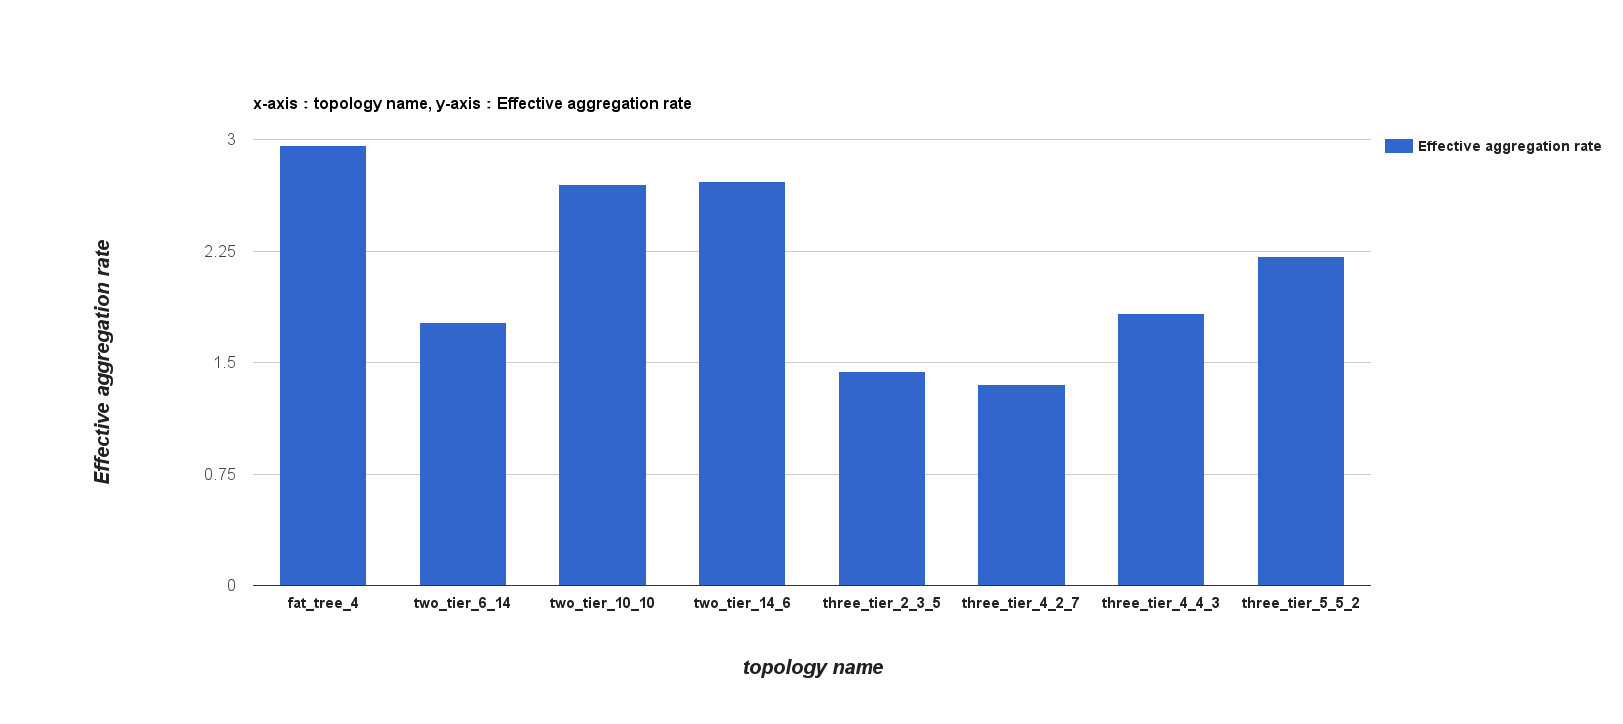
\includegraphics[width=1.4\linewidth]{figures/exp_topotype_bar.png}
\end{center}
\caption{The bar chart of different topologies.}
\label{different_topo_bar}
\end{figure}



We select the most effective one, fat\_tree\_4, and the least effective one, three\_tier\_4\_2\_7, for further examination with the distribution of the number of entry contained in each group, shown as Figure~\ref{different_topo_distribute}. From the figure, we can see two things: first, a lot of groups in three\_tier\_2\_7 only contain one entry. XXXXXXXXXXXXXXXXXXXXX
Second, the area coverage of three\_tier\_4\_2\_7 is apparently larger than fat\_tree\_4. This can mean that the groups contain either a lot more auxiliary entries or redundant entries caused by the entries with same match field an value, or even both. 

In order for further inspection, XXXXXXXXXXXX.
\begin{figure}[H]
\begin{center} 
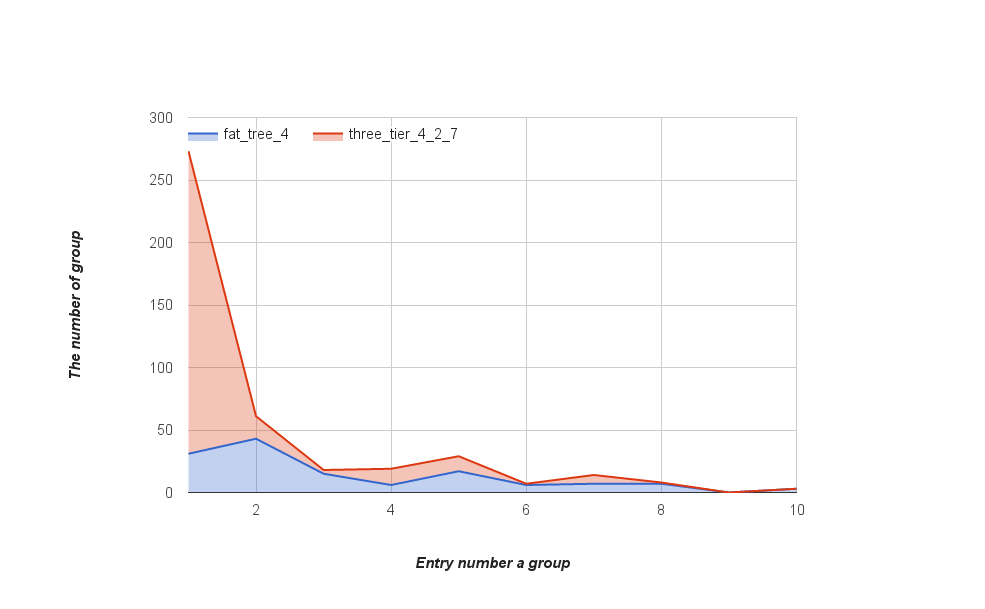
\includegraphics[width=1.4\linewidth]{figures/exp_topotype_distribute.png}
\end{center}
\caption{The comparison between .}
\label{different_topo_distribute}
\end{figure}

\subsection{Influence of network scale}
To observe how effective our method is under different network scales, different size of fat tree topology will be used. Since the network scale grows significantly with higher pod number(the only parameter fat tree topologies have), we will only have from fat\_tree\_2 to fat\_tree\_14. There are also 20 entries on each switch.

The result is in Table~~\ref{table:different_scale}

\begin{table}
\centering
\caption{Influence of different network scales}
\begin{tabular}{|l||l|l|l|l|}
\hline topology name & Effective aggregation rate & Actual aggregation rate & Execution time(sec) & Number of auxiliary entry \\
\hline
\hline fat\_tree\_2 & 2.70 & 2.84 & 1.26 & 35 \\
\hline fat\_tree\_4 & 2.96 & 3.27 & 8.27 & 142 \\
\hline fat\_tree\_6 & 2.85 & 3.27 & 19.16 & 327 \\
\hline fat\_tree\_8 & 2.81 & 3.29 & 33.03 & 589 \\
\hline fat\_tree\_10 & 2.91 & 3.37 & 51.81 & 921 \\
\hline fat\_tree\_12 & 2.89 & 3.36 & 74.78 & 1334 \\
\hline fat\_tree\_14 & 2.79 & 3.29 & 102.56 & 1800 \\
\hline
\end{tabular}
\label{table:different_scale}
\end{table}

As we can see from the trend chart of effective aggregation rate and actual aggregation rate in Figure~\ref{different_scale_rate_trend}, XXXXXXXXXXX.

\begin{figure}[H]
\begin{center} 
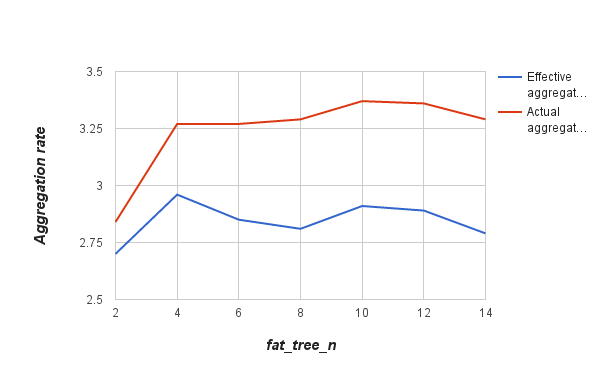
\includegraphics[width=1\textwidth]{figures/exp_scale_rate_trend.png}
\end{center}
\caption{The trend chart of aggregation rates under different scale of network.}
\label{different_scale_rate_trend}
\end{figure}



The trend of execution time and number of auxiliary entries while increasing the network scale are shown as Figure~\ref{different_scale_time_trend} and Figure~\ref{different_scale_aux_trend}. 


Since an auxiliary entry is needed for every entry leads to a host, and the , the number of the auxiliary entries 
XXXXXXXXXX.


\begin{figure}[H]
\begin{center} 
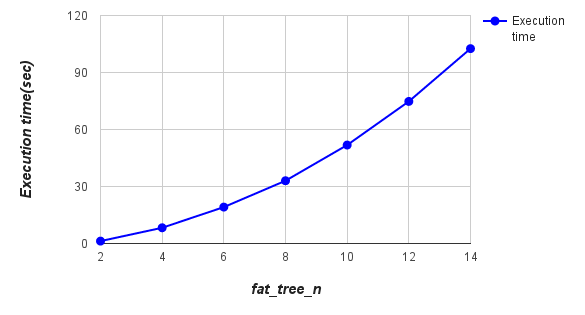
\includegraphics[width=1\textwidth]{figures/exp_scale_time_trend.png}
\end{center}
\caption{The trend chart of execution time under different scale of network.}
\label{different_scale_time_trend}
\end{figure}



\begin{figure}[H]
\begin{center} 
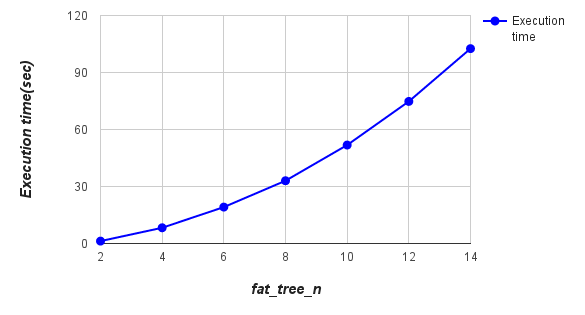
\includegraphics[width=1\textwidth]{figures/exp_scale_time_trend.png}
\end{center}
\caption{The trend chart of number of auxiliary entries under different scale of network.}
\label{different_scale_aux_trend}
\end{figure}



\subsection{Influence of flow entry number}
In this experiment, we will use only one topology - fat\_tree\_4 and change the number of entries on each switch to see the influence it might bring. The number of entries on each switch are from 5 to 50, with 5 entries increasing every run. The result table is in Table~~\ref{table:different_entry_per_switch}. The execution time and the number of auxiliary grow linearly, which is quite expected since the number of entry also grows linearly.

\begin{table}
\centering
\caption{Different number of entries in a switch.}
\begin{tabular}{|l||l|l|l|l|}
\hline Number of entries per switch & Effective aggregation rate & Actual aggregation rate & Execution time (sec) & Number of auxiliary entry \\
\hline
\hline 5 & 2.27 & 2.66 & 1.64 & 36 \\
\hline 10 & 2.38 & 2.82 & 3.98 & 72 \\
\hline 15 & 2.59 & 2.91 & 5.53 & 110 \\
\hline 20 & 2.96 & 3.27 & 8.27 & 142 \\
\hline 25 & 2.94 & 3.29 & 11.08 & 179 \\
\hline 30 & 3.14 & 3.55 & 15.03 & 214 \\
\hline 35 & 3.19 & 3.58 & 17.22 & 242 \\
\hline 40 & 3.36 & 3.72 & 19.24 & 280 \\
\hline 45 & 3.37 & 3.80 & 24.42 & 310 \\
\hline 50 & 3.45 & 3.86 & 26.19 & 346 \\
\hline
\end{tabular}
\label{table:different_entry_per_switch}
\end{table}

The trend chart Figure~\ref{exp_entrynum_trend} shows that XXXXXXXXXXXXXX. 

\begin{figure}[H]
\begin{center} 
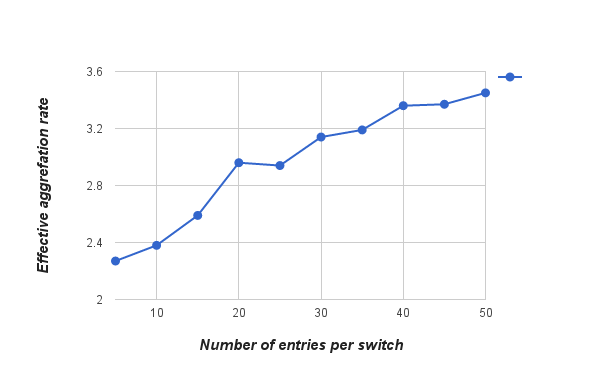
\includegraphics[width=1\textwidth]{figures/exp_entrynum_trend.png}
\end{center}
\caption{The trend chart of different number of entries on every switch.}
\label{exp_entrynum_trend}
\end{figure}

\subsection{Sum up for experimental results}
-------------------------
However, the aggregation rates do not always grow along with the scale of the network. The reason is that XXXXXXXXXXXXX.


The degree of switch is particularly to our method because the higher the degree is, the higher the chance of finding more entries in an aggregated group will be.


factors that influence the result:
	-link number
	-the number of host/edge switch
	-scatter 
	-overlapping same (f,v) set

%host number = k^3 / 4
\chapter{Conclusion and future work}
\label{conclusion}
In this work, we discuss the hazard that an compromised switch in SDN network may bring. In the scenario we set up, we can see how the problems can be solved by using SDN features. Even a different scenario is met, we believe that the new problems it introduces can also be solved with some extension and adjustment with the functionality SDN provides. We propose an effective way that is able to scan through the entire network for disobedient forwarding behavior with less number of packets, and evaluate it under different network topology types, scales and entry numbers on each switch. The experimental result demonstrates that our method is effective under a network topology with balance structure. Also, the scale of the network topology does not affect the efficiency significantly, and the aggregation rate grows to 3.48 in fat tree topology once there are 120 entries in each switch. 

We can only anticipate what the attackers may try to target with SDNs. The deployments are new, the protocols are new, the controller software is new, and the history of past SDN attacks is unknown. Based on the SDN architecture, we can predict where an attacker may be likely to strike. If we put ourselves in the attacker\textquotesingle s shoes, we might be able to spot a weakness to exploit. Then we can harden that weakness ahead of time. Before an organization embarks on an SDN deployment project, they should consider how they would secure the system during the early design stage. 

In the future work, more realistic factors should be taken into consideration, such as the collaboration of multiple compromised switches and the entries with multiple match fields and wildcard fields. Furthermore, the aggregated group finding method currently performs DFS without any estimation, the core algorithm can be improved by adding heuristic function. Also, as the new versions of OpenFlow are released, the method should be able to be optimized with the support of the new features. For example, the auxiliary entries can be installed on the egress table once it is fully supported.

\begin{thebibliography}{1}

\bibitem{KRVRAU15} %journal
D. Kreutz, F. M. Ramos, P.E. Verissimo, C.E. Rothenberg, S. Azodolmolky and S. Uhlig,
``Software-Defined Networking: A Comprehensive Survey,'' In Proceeedings of the IEEE, vol. 103, no. 1, pp.  14-76, Jan. 2015.

\bibitem{MABPPRST08}
N. McKeown, T. Anderson, H. Balakrishnan, G. Parulkar, L. Peterson, J. Rexford, S. Shenker and J. Turner,
``OpenFlow: Enabling Innovation in Campus Networks,'' ACM SIGCOMM Computer Communication Review, vol. 38, issue 2, pp. 69-74, Apr. 2008.

\bibitem{LHM10} %conf
B. Lantz, B. Heller and N. McKeown,
``A Network in a Laptop: Rapid Prototyping for Software-Defined Network,'' In Proc. of the 9th ACM SIGCOMM Workshop on Hot Topics in Networks, Oct. 2010.

\bibitem{OF_SPEC}
OpenFlow Switch Version 1.5 Specification, \url{https://www.opennetworking.org/images/stories/downloads/sdn-resources/onfspecifications/openflow/openflow-switch-v1.5.1.pdf}.

\bibitem{SOS13}
S. Scott-Hayward, G. O’Callaghan and S. Sezer,
``SDN Security: A Survey,'' In Proc. of IEEE SDN for Future Networks and Services (SDN4FNS), pp. 1–7., Nov. 2013.

\bibitem{CM}
M. Coughlin,
``A Survey of SDN Security Research,'' \url{http://ngn.cs.colorado.edu/~coughlin/doc/a_survey_of_sdn_security_research.pdf}.

\bibitem{HXWG15}
S. Hong, L. Xu, H. Wang and G. Gu,
``Poisoning Network Visibility in Software-Defined Networks: New Attacks and Countermeasures,''  In Proceedings of the 22th Annual Network and Distributed System Security Symposium (NDSS), Feb. 2015.

\bibitem{CKGL15}
P. W. Chi, C. T. Kuo, J. W. Guo and C. L. Lei,
``How to Detect a Compromised SDN Switch,'' In Proc. of the 1st IEEE Conference Network of Softwarization (NetSoft), pp. 1-6., Apr. 2015.

\bibitem{PJL16}
C. Pang, Y. Jiang and Q. Li,
``FADE: Detecting Forwarding Anomaly in Software-Defined Networks,'' In Proc. IEEE International Conference of Communications (ICC), May 2016.

\bibitem{ZKVM12}
H. Zengyz, P. Kazemianyz, G. Varghese and N. McKeowny,
``Automatic Test Packet Generation,'' In Proc. of the 8th International Conference on Emerging Networking Experiments and Technologies (CoNEXT), Dec. 2012.

\bibitem{HP_SPEC}
HP OpenFlow 1.3 Administrator Guide, \url{http://h10032.www1.hp.com/ctg/Manual/c04495114}.

\bibitem{OVS_OFCTL}
OpenvSwitch Manual, \url{http://openvswitch.org/support/dist-docs/ovs-ofctl.8.txt}.

\bibitem{LAB14}
L. Schehlmann, A. Sebastian and B. Harald, 
``Blessing or curse? Revisiting security aspects of Software-Defined Networking,'' In Proc. of 10th IEEE International Conference on Network and Service Management (CNSM), Nov. 2014.

\bibitem{KJK}
A. Khandelwal, N. Jain and S. Kamara,
``Attacking Data Center Networks from the Inside,'' \url{https://www.microsoft.com/en-us/research/wp-content/uploads/2016/02/dcn.pdf}.

\bibitem{TTB15}
T. THANH BUI,
``Analysis of Topology Poisoning Attacks in Software-Defined Networking,'' Degree project in security and mobile computing, Second Level Stockholm, Aug. 2015.

\bibitem{ATPP15}
T. Alharbi, M. Portmann and F. Pakzad,
``The (In) Security of Topology Discovery in Software Defined Networks,'' In Proc. of 40th IEEE Conference on Local Computer Networks (LCN), Oct. 2015.
 
\bibitem{AAS14}
M. Antikainen, T. Aura and M. Särelä,
``Spook in Your Network: Attacking an SDN with a Compromised OpenFlow Switch,'' In Proc. of Nordic Conference on Secure IT System (NordSec), Oct. 2014.

\bibitem{ARDC14}
K. Agarwal, E. Rozner, C. Dixon and J. Carter,
``SDN traceroute: Tracing SDN Forwarding without Changing Network Behavior,'' In Proc. of the 3rd ACM Workshop on HotTopics in Software Defined Networking (HotSDN), Aug. 2014.

\bibitem{BCKK15}
R. Bifulco, H. Cui, G. O. Karame and F. Klaedtke,
``Fingerprinting software-defined networks,'' In Proc. of 2015 IEEE 23rd International Conference on Network Protocols (ICNP), Nov. 2015.

\bibitem{DMR97}
D. Karger, M. Rajeev and G. D. S. Ramkumar,
``On approximating the longest path in a graph,'' in Algorithmica, pp. 82-98, May 1997.

\bibitem{RU04}
R. Uehara and Y. Uno,
``Efficient algorithms for the longest path problem,'' in Algorithms and Computation, Springer Berlin Heidelberg, pp. 871-883, Dec. 2005.


\bibitem{Mininet}
Mininet Official Website, \url{http://mininet.org/}.

\bibitem{FNSS}
Topology Package In FNSS API Documentation, \url{http://fnss.github.io/doc/core/apidoc/fnss.functions.html#topologies-package}.

\bibitem{PACKETOUT}
Flowgrammable SDN OpenFlow Doumentation Message-Layer Section, \url{http://flowgrammable.org/sdn/openflow/message-layer/packetout/}.

\bibitem{MPFHMRSV09}
R. Niranjan Mysore, A. Pamboris, N. Farrington, N. Huang, P. Miri, S. Radhakrishnan, V. Subramanya and A. Vahdat, ``PortLand: A Scalable Fault-Tolerant Layer 2 Data Center Network Fabric,'' ACM SIGCOMM Computer Communication Review, Vol. 39, no. 4, pp. 39-50., Aug. 2009.

\bibitem{PORT_FREQ}
Network Traffic Breakdown By Protocol Discussion On WhatPulse, \url{http://dkqnkzjkqr9h2.cloudfront.net/forums/showthread.php?tid=6987}.
\end{thebibliography}
\end{document}